
% Chapter6
\tocdata{toc}{Di Wan}

\chapter{Recommendation Engine}% Main chapter title
\label{Chapter6} % Change X to a consecutive number; for referencing this chapter elsewhere, use \ref{ChapterX}

\section{Introduction}
A recommendation engine is a data filtering tool using machine learning algorithms to recommend the most relevant items to a particular user or customer. It operates on finding patterns in consumer behaviour data, which can be collected implicitly or explicitly. In our case, the quality of the recommendation system design determines the quality of the posts recommended to our users. We include a recommendation engine to recommend posts, in our case, songs created and shared by our users to each individual user.
\\A recent study by Epsilon\footnote{Epsilon. (2018, April 11). The personalisation mismatch: Rift grows between brand offerings and consumer desires. geo-redirect. Retrieved May 15, 2022, from https://www.epsilon.com/emea/about-us/pressroom/epsilon-report }, found that 90\% of consumers find personalisation appealing. A further 80\% claim they are more likely to cooperate with a company when offered personalised experiences.
The study also found that these consumers are ten times more likely to become VIP customers who make more than 15 purchases per year.
Thus, a well-designed recommendation system can benefit the monetisation of our app in the future.
\\Recommendation systems are divided into personalised and non-personalised systems, where personalised recommendation systems can be further divided into content-based and collaborative filtering systems. 
The overview of the recommendation system can be seen in \cref{fig:overrecomm}. In this chapter, we will discuss the working theory of each system, and analyse the applicability to our design and problems we may face and possible solutions we had.
\begin{figure}[ht]
\centering
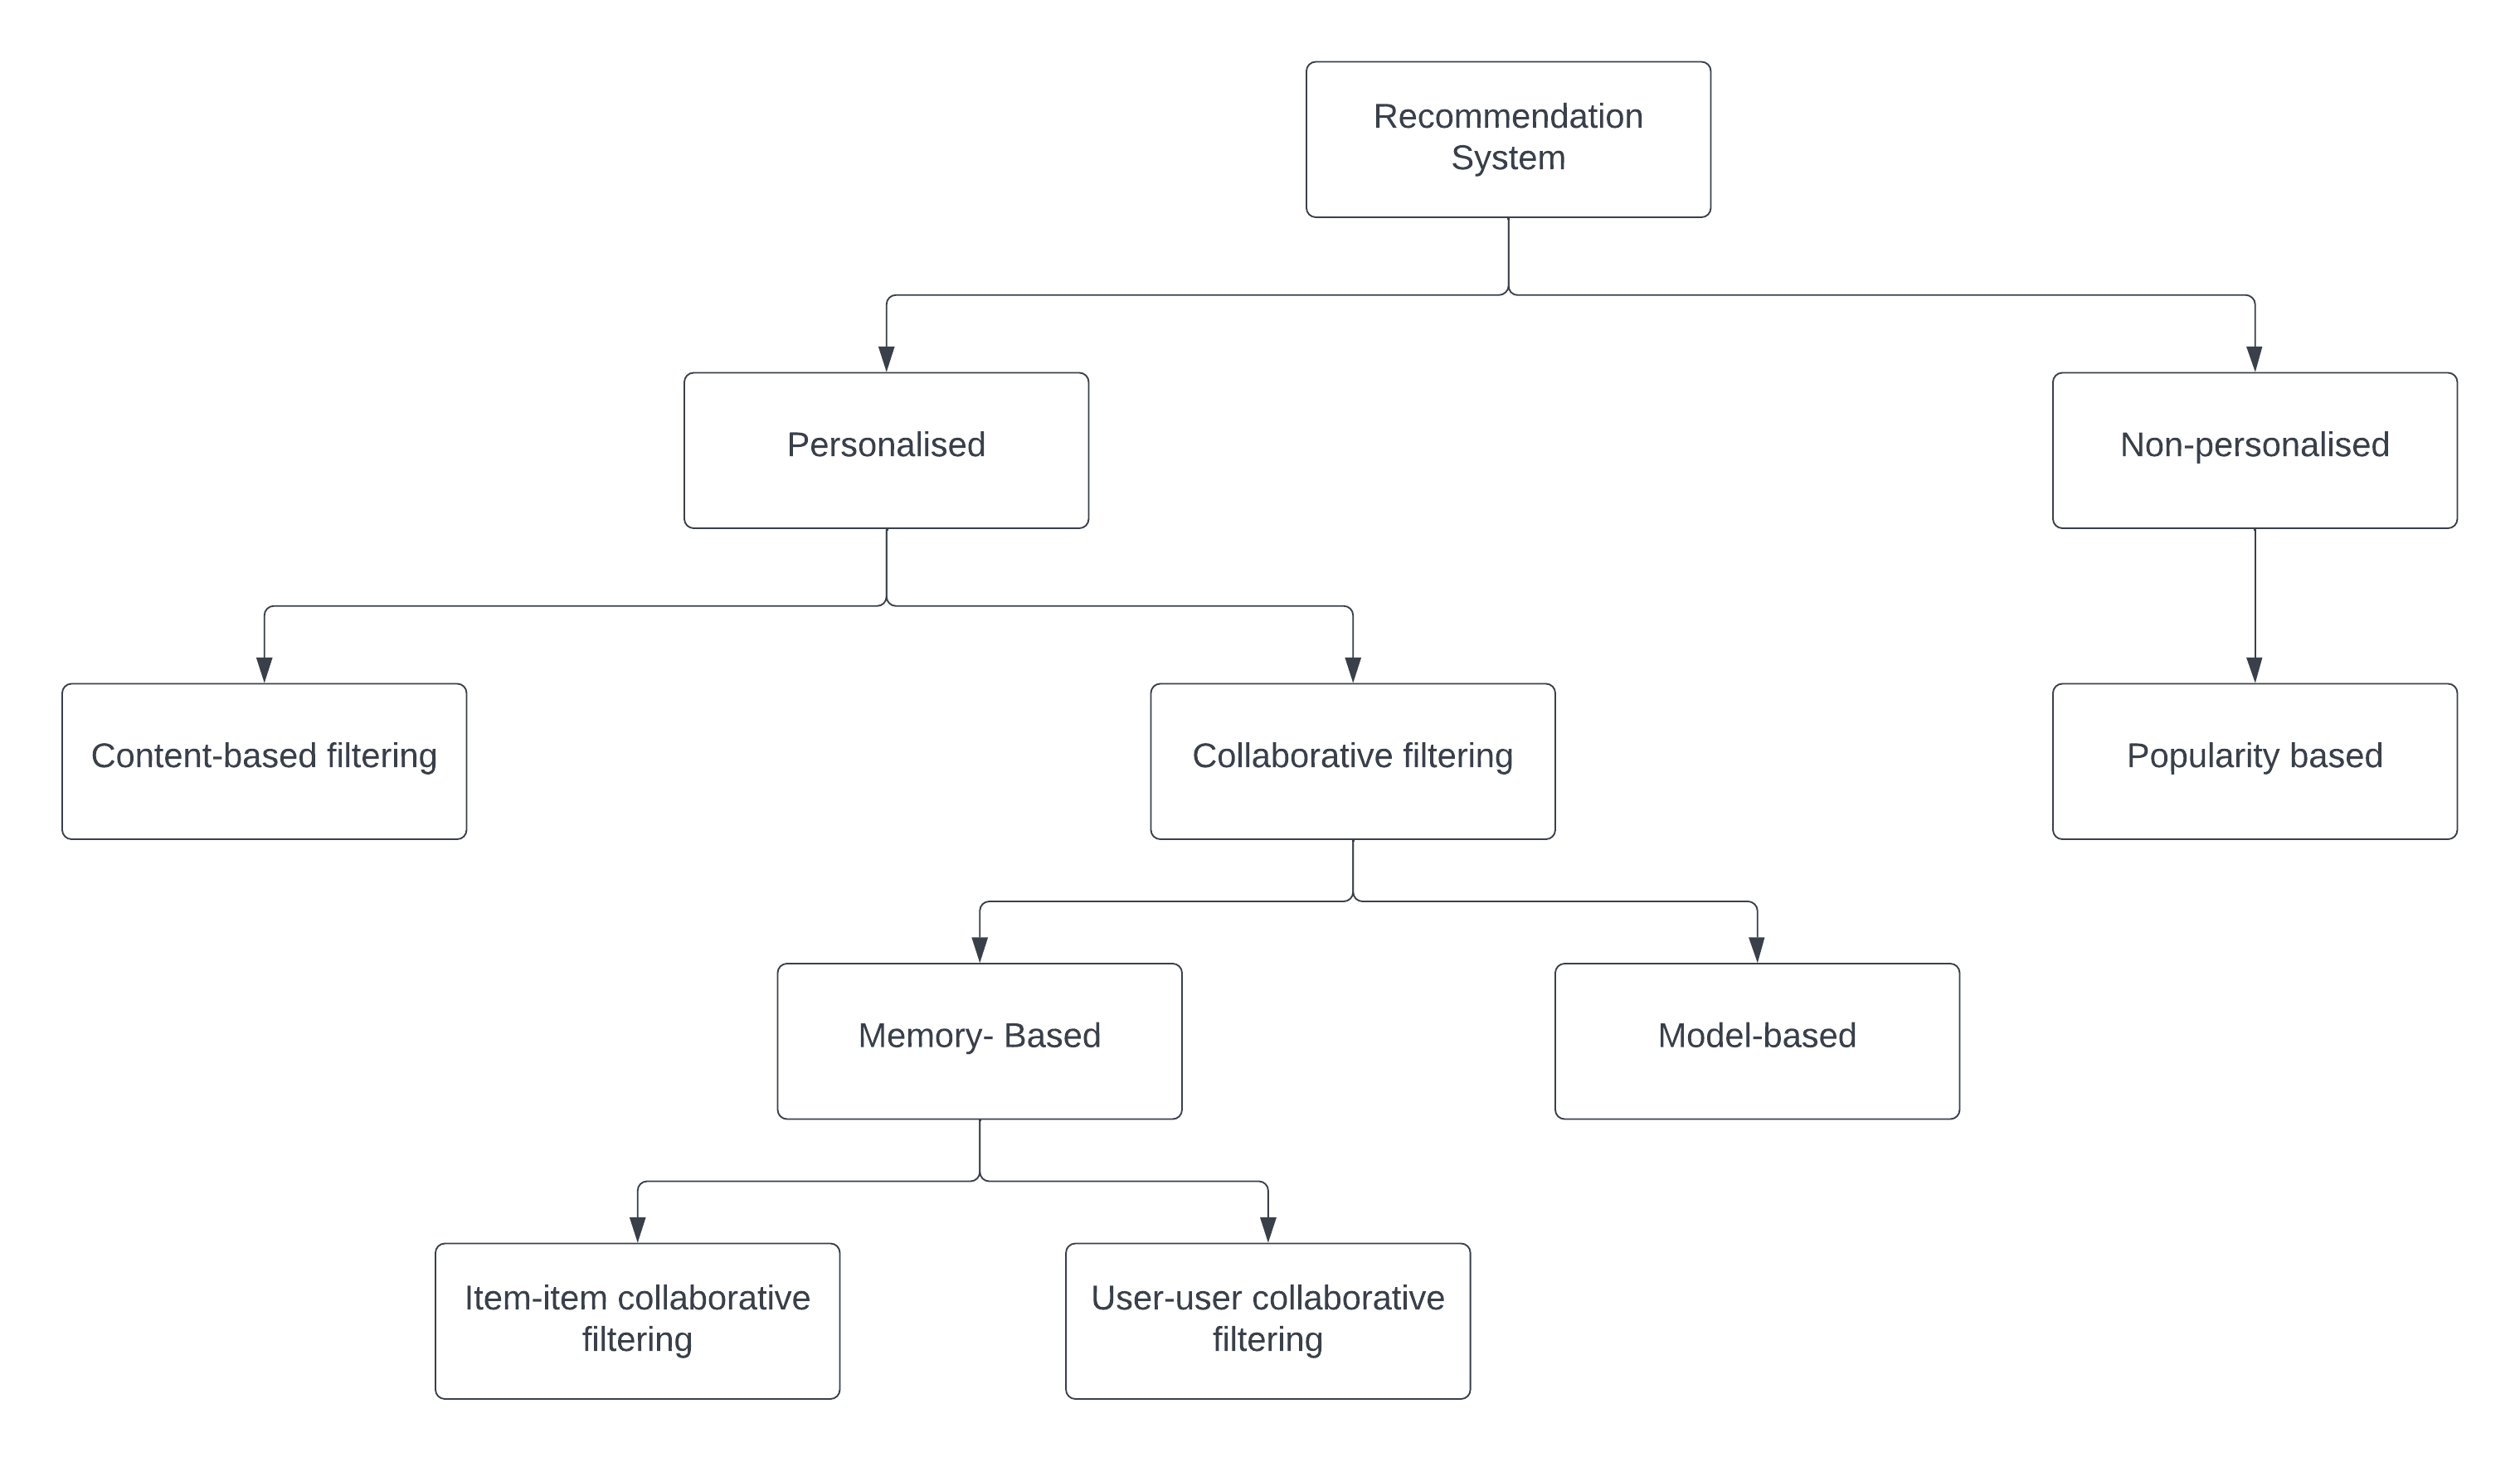
\includegraphics[width=0.8\columnwidth]{overview11.png}
\caption{Overview of recommendation system}
\label{fig:overrecomm}
\end{figure}

%-----------------------------------------------------------------------------------------------------------------------------Popularity-Based Recommendation System
\section{Popularity-based Recommendation System}
Popularity-based recommendation system works on the principle of popularity or anything in trend. These systems check the items in trend or are most popular among the users and directly recommend those. 
For our design, instead of recommending posts only based on the number of likes that the posts received, we can give weighting to each parameter involved in our decision. One of the weighted rating models we constructed is shown below.
\begin{equation*}
\text{Rating} = f(L,C,m,g,T) = \alpha \times \frac{L^{2}}{L+m} + \beta \times \frac{C^{2}}{C+m} + T \times g_{[k-2,k]}
\end{equation*}
Where:
\\$L$ is the number of likes the post received.
\\$C$ is the number of comments the post received.
\\$m$ is the minimum of like preferences required to be listed as a popular item.
\\$g_{[k-2,k]}$ is the gradient of change in the total number of likes and comments in w.r.t time in the last two days, which is calculated by 
$g_{[k-2,k]} = \frac{L_{k} + C_{k} -L_{k-2} -C_{k-2}}{2}$, with $k$ indicates \textit{the current day} and $(k-3)$ indicates \textit{three days ago}.
\\$T$ is the period and we set $T=1$.
\\ $\alpha$ and $\beta$ are constants.
\\This formula is a modified version based on the rating system by IMDB\footnote{Seeda, P. (2021, October 13). A complete guide to recommender system-tutorial with Sklearn, surprise, Keras, Recommender. Medium. Retrieved May 15, 2022, from https://towardsdatascience.com/a-complete-guide-to-recommender-system-tutorial-with-sklearn-surprise-keras-recommender-5e52e8ceace1}, which is an online database of information related to films and television series. We introduced non-linearity in the weightings for $L$ and $C$, and it can be seen that we set a threshold for these two parameters; for example, if $L \gg m$, then the first term on the right-hand side will be dominated by $L$, same for $C$ in the second term. The non-linearity here is to attenuate the contribution brought by $L$ and $C$ when these values are small. The last term on the right-hand side predicts the increase in the total number of likes and comments for the next day, assuming the gradient change the day after is the same as two days ago. The further improvement we made is introducing $\alpha$ and $\beta$ to indicate the relative significances of $L$ and $C$, and it is usually considered that $L$ is more significant than $C$, so $\alpha > \beta$. Finally, the system will rank and recommend the posts by the ratings.
\\The advantage of the popularity based system is that it is easy to implement and requires relatively low computational power. However, the most apparent disadvantage of a popularity-based system is the non-personalisation because it does not analyse the individual user's preference. 


%-----------------------------------------------------------------------------------------------------------------------------Content-Based Recommendation System
\section{Content-based Recommendation System}
\label{Content Based Recommendation System}
Content-based recommendation systems depend on a profile of the user's preferences and feature descriptions of the item.
The recommendation is modelled as a user-specific classification problem that estimates users' likes and dislikes based on an item's features with a content-based recommender.
\\ The system requires the post-feature matrix (\cref{itemfea}) to be constructed for all posts in our case, and we assume that there are available features (mood, time length, etc.) that capture the content of the post. The ratings that are given in the table measure the degree of the features in the posts, and we can assume the matrix is not sparse, which means the matrix is fully filled. And we denote that each row is the feature vector $x_i$ for post $i$.
\begin{table}[ht]
\centering
\begin{tabular}{ |c|c|c|c|c|c|} 
 \hline
 \diagbox{Posts}{Features}&Feature1&Feature 2&Feature 3&$\cdots$&Feature $k$\\
 \hline
 Post1&&&&&\\
 \hline
 Post2&&&&&\\
 \hline
 $\vdots$&&&&&\\
 \hline
 Post $i$&&&&&\\
 \hline
 \end{tabular}
 \caption{Post Feature Matrix}
 \label{itemfea}
 \end{table}
\\In addition, we need to get the profile of each user, which means we need to know and analyse the preferences of our users, so we need to obtain the user parameter vector for each user, reflecting how the user responds to the features. \cref{userpa} shows the user parameter matrix, and we denote each row is the user parameter vector $\theta_j$ for user $j$. 
\begin{table}[ht]
\centering
\begin{tabular}{ |c|c|c|c|c|c|} 
 \hline
 \diagbox{Users}{Features}&Feature1&Feature 2&Feature 3&$\cdots$&Feature $k$\\
 \hline
 User 1&&&&&\\
 \hline
 User 2&&&&&\\
 \hline
 $\vdots$&&&&&\\
 \hline
 User $j$&&&&&\\
 \hline
 \end{tabular}
 \caption{User Parameter Matrix}
 \label{userpa}
 \end{table}
\\After we have the post-feature matrix and the user parameter matrix, we apply similarity metrics, and we chose \textit{cosine similarity} to measure the resonance between each combination of $\theta_j$ and each $x_i$. Cosine Similarity, as the name mentioned, it measures the cosine angle of the two vectors in the multidimensional space. Two things can be similar together in terms of direction rather than magnitude.
\begin{equation*}
\text{Cosine Similarity} = cos(\theta) = \frac{A \cdot B}{||A|| ||B||}
\end{equation*}
\\Finally, the system can rank and recommend posts to user $k$ based on the similarity scores between $\theta_j$ and each $x_i$.

\subsection*{Problems and Possible Solutions}
The biggest challenge with this approach in our design is to determine the content's subjective features, such as genre, vibe, mood, etc. Our current solution to this problem is by including the “feature tags” in the posts, and we will give a limited number of choices for our users to choose from 
with a percentage meter to indicate the degree of the features. Therefore, the post-feature matrix will rely on our users, which may suffer from subjectivity. It is based on the assumption that our users are unlikely to lie about the features of their own songs. We believe this design gives our users more freedom and space to show the feelings behind their songs so that it may improve the user experience. 
%
\subsection*{Advantages}
\begin{itemize}
\item Content-based models are able to provide recommendations without knowing any information about other users, such as their preferred features and liked posts.
\item Extended from the previous advantage, since the system treats recommendations for each individual user as an isolated task from each other, the system can capture the specific interest of a user, and recommend niche posts that few other people are interested in.
\end{itemize}

\subsection*{Disadvantages}
\begin{itemize}
\item One of the disadvantages is that the systems are ineffective in providing recommendations for new users because the system does not have the parameter vectors for the new users. 
The solution to it can be through a UX/UI design, which is inspired by Apple Music, YouTube Music and Xiaohongshu\footnote{Wikimedia Foundation. (2022, April 23). Xiaohongshu. Wikipedia. Retrieved May 15, 2022, from https://en.wikipedia.org/wiki/Xiaohongshu }. We would pop out a page for our users to choose preferred features from given choices, and the bubbles will have three sizes to indicate 'interested in', 'like' and 'very like' levels of preferences. After users select, our system will initialise the user parameter vectors, and it helps solves the initialisation problem.%\item Another disadvantage can be that it requires a history of explicit/implicit user-level data for the items when building a model. It’s generally essential to have a large dataset of ratings available to make robust predictions without overfitting.  
\item The recommendations provided are “obvious” based on the posts/content the user has interacted with before. This is a disadvantage because if the user has never interacted with a particular type of post, that type will never be recommended to the user. 
For example, if the user has not seen any sad song post, then through this approach, he will never be recommended sad song posts. This is because the model is user-specific and doesn’t leverage knowledge from similar users. This reduces the diversity of the recommendations.
%
\item Also, people's preferences will change, but the content-based approach does not provide a way to update user parameter vectors. Considering user experience, we can not ask our users to update their preferences every day or week. Out-of-date user parameter vectors can lead to inefficient recommendations, further affecting our user experience. Thus being incapable to update the user parameter vector is also $y_{ij}$one of the drawbacks of this approach.
\end{itemize}



%-----------------------------------------------------------------------------------------------------------------------------Collaborative Recommendation System
\section{Collaborative Filtering Recommendation System}
Collaborative filtering predicts users' interests by identifying preferences and information from many users.\footnote{Recommendation Systems Explained. Explaining \& Implementing Content .... https://towardsdatascience.com/recommendation-systems-explained-a42fc60591ed} 
This is done by filtering data for information or patterns using techniques involving collaboration among multiple agents, data sources, etc. 
The underlying intuition behind collaborative filtering is that if user A and B have similar tastes in an item, then A and B are likely to have similar tastes in other items. We can divide the collaborative filtering system into a model-based approach and a memory-based approach. The memory-based approach can further be divided into item-based and user-based systems. A clear structure can be seen in \cref{fig:overrecomm}.
\\The first step through collaborative filtering to our design is to construct the user-post interaction matrix. (\cref{fig:UtilityM})
\begin{table}[ht]
\centering
\begin{tabular}{ |c|c|c|c|c|c|} 
 \hline
 \diagbox{posts}{Users}&User 1&User 2&User 3&$\cdots$&User $j$\\
 \hline
 post1&&&&&\\
 \hline
 post2&&&&&\\
 \hline
 post3&&&&&\\
 \hline
 $\vdots$&&&&&\\
 \hline
 post $i$&&&&&$y_{ij} \text{ if } r_{ij} = 1$\\
 \hline
 \end{tabular}
 \caption{User-post Interaction Matrix}
 \label{fig:UtilityM}
 \end{table}
\\We denote that: $r_{ij}$ is a boolean value and $r_{ij} = 1$,  if user $j$ rated item $i$ ($0$,  otherwise). And $y_{ij}$ is the rating by user $j$ on item $i$.
\\The first challenge that will be faced in this approach is how we can get ratings $y_{ij}$. The music posts are different from the movie rating system; considering our user experience, we cannot ask our users to rate each post. 
The more sensible way is to allow them to give “Likes”. However, inspired by a Chinese video-streaming app, Bilibili, we can make some changes to the “like” system. 
Instead of “like” or “not give like”, we introduce a “super like” that our user can give to a post by 'pressing and holding the 'like' button.
\\Now we want to construct a rating function $y_{ij}(L,t,S,T)$ where, 
\begin{itemize}
\item$L$ is 0 if “no like is given”, 1 if “liked”, and 2 if “super liked”.
\item$t$ is the time our user spent on the post. Since we are not introducing a “dislike” feature in posts that discourage our users from sharing their works, we will set a threshold value for indicting “dislike”. For example, if a user spends 3 seconds, below the threshold value, on a post and then exits, the system will turn $L$ into ”-1”.
\item$S$ is 0 if the user and 1 have not saved the post if the user saves the post.
\item$T$ is how many times the user $j$ has watched post $i$.
\end{itemize}
The formula we want to construct considers both explicit and implicit information. Formulating the equation can be another big problem; like in machine learning, we need a large dataset to fit our model or function into, which means we need to get ratings to test or validate our rating function. The solution to it has not been clear because of the project time length.

%-----------------------------------------------------------------------------------------------------------------------------Memory-based CF
\subsection{Memory Based Approaches}
Memory-based approaches are also often referred to as neighbourhood collaborative filtering. Essentially, ratings of user-post combinations are predicted based on their neighbourhoods. The memory-based approach is simple since it just calculates the similarity matrix directly from the user-item matrix. There are two branches of memory-based approaches: item-based and user-based collaborative filtering. User-based essentially means that like-minded users will yield strong and similar recommendations. Item-based collaborative filtering recommends items based on the similarity between items calculated using user ratings of those items.
\subsubsection{Item-based Collaborative Filtering}
This method was first invented and used by Amazon in 1998. We can use item-to-item collaborative filtering to match each user’s liked posts to similar posts and then combines those similar posts into a recommendation list.
We can use item-to-item collaborative filtering to match each user’s liked posts to similar posts and then combines those similar posts into a recommendation list.
Instead of applying cosine similarity, the better approach will be using the Pearson correlation coefficient, the most well-known similarity metric for the linear relation. It measures the similarity between two samples based on the direction of how the value changes. It is also called \textbf{Centred Cosine Similarity}, and the word “Centred” means we will normalise the Utility matrix first by subtracting the row mean. Compared to cosine similarity, Pearson Correlation solves the problem when we assume unwatched posts by the user to be rated 0. The assumption is considered not much reasonable.
\begin{equation*}
\text{Pearson Correlation Coefficient} = \frac{\sum(x_{i} - \bar{x})(y_{i} - \bar{y})} {\sqrt{\sum(x_{i} - \bar{x})^{2} \sum{(y_{i} - \bar{y})^{2} }}}
\end{equation*}


\subsubsection{User-based Collaborative Filtering}
In this approach, we find the group of similar users based on the Pearson correlation similarity metric. Then we average the rating of each item based on the group of similar users. Finally, the system can rank the item based on the descending average rating and recommend the target user with the item they never interacted with before.

%-----------------------------------------------------------------------------------------------------------------------------Model-based CF
\subsection{Model-based Approaches}
Model-based approaches are predictive models using machine learning. Features associated with the dataset are parameterised as inputs of the model to try to solve an optimisation related problem. The idea behind it is that we believe that we can decompose the Utility matrix into two latent factor matrices, in our case, the user-parameter latent matrix and the post-feature latent matrix. And we will be able to predict the missing ratings in the original Utility matrix by reconstructing it by multiplying two latent matrices together. This is done by Matrix factorisation, which will be explained later in section \ref{Matrix Factorisation}.
\subsubsection{Optimisation Algorithm}
The algorithm explanation here is mostly based on Dr Andrew Ng's Machine Learning Course.\footnote{Ng, A. Y.-T. (2017, February 9). Lecture 16.1 - recommender systems | problem formulation - [ machine learning | Andrew Ng ]. YouTube. Retrieved May 15, 2022, from https://www.youtube.com/watch?v=giIXNoiqO\_U} Firstly, we need to construct the user-post interaction matrix. (\cref{fig:UtilityM})
\begin{enumerate}
\begin{table}[ht]
\centering
\begin{tabular}{ |c|c|c|c|c|c|} 
 \hline
 \diagbox{Posts}{Users}&User 1&User 2&User 3&$\cdots$&User $j$\\
 \hline
 Post1&&&&&\\
 \hline
 Post2&&&&&\\
 \hline
 Post3&&&&&\\
 \hline
 $\vdots$&&&&&\\
 \hline
 post $i$&&&&&$y_{i,j} \text{ if } r_{i,j} = 1$\\
 \hline
 \end{tabular}
 \caption{User-Post Interaction Matrix}
 \centering
 \end{table}

\item We need to obtain a set of feature folders, each is measuring the degree of the content.
Denote that:
\\$r_{ij}$ is a boolean value and $r_{ij} = 1$, if user $j$ rated item $i$ ($0$, otherwise.)
\\$y_{ij}$ \text{is the rating by user $j$ on item $i$}
\\$\theta_{j}$ \text{is the parameter vector of user $j$}, which is a latent-factor
\\$x_{i}$ \text{is the feature vector of item $i$}, which is a latent-factor
\\$m_{j}$ \text{is the number of items rated by user $j$}
\\We want to reconstruct the matrix and compute the absent ratings using matrix factorisation, then the predicted rate on the item $i$ by user $j$ is $(\theta_{i})^{T}(x_{j})$
\item We treat predicting the ratings of each user as a separate linear regression problem.
\item We try to minimise the square error term.
\end{enumerate}
Thus, if we want to learn $\theta_{i}$ for user $j$:

\begin{equation*}
\min_{\theta_{j}} \frac{1}{2m_{j}}\sum_{i:r_{i,j} = 1}\left((\theta_{i}^{T}x_{i}-y_{ij}\right)^{2} + \frac{\lambda}{2m_{j}}\sum_{k = 1}^{n}(\theta_{ik})^{2}
\end{equation*}
\\Where the last term is the usual regularisation term to prevent the overall equation from going to infinity and preventing overfitting.
\\To learn $\theta_{1}$,$\theta_{2}$, \dots, $\theta_{j}$:
\begin{equation}
\label{eqq111}
\min_{\theta_{1},\theta_{2}, \dots, \theta_{j}} \frac{1}{2}\sum_{j = 1}^{n_{u}}\sum_{i:r_{i,j} = 1}\left((\theta_{i})^{T}x_{j}-y_{ij}\right)^{2} + \frac{\lambda}{2}\sum_{j = 1}^{n_{u}}\sum_{k = 1}^{n}(\theta_{ik})^{2}
\end{equation}
\\where $n_{u}$ is number of users, and we get rid of term $m_{j}$ because it is a constant which will not affect the result when we proceed the optimisation.
\\Similarly, if we are given $\theta_{1}$,$\theta_{2}$, \dots, $\theta_{j}$, to learn $x_{1}$,$x_{2}$,\dots,$x_{i}$:
\begin{equation}
\label{eqq222}
\min_{x_{1},x_{2}, \dots,x_{j}} \frac{1}{2}\sum_{i = 1}^{n_{m}}\sum_{i:r_{i,j} = 1}\left((\theta_{i})^{T}x_{j}-y_{ij}\right)^{2} + \frac{\lambda}{2}\sum_{j = 1}^{n_{m}}\sum_{k = 1}^{n}(\theta_{ik})^{2}
\end{equation}
\\Where the last term is usual regularisation term to prevent the overall equation to go to infinity, to prevent overfitting.
\\The objective of our collaborative optimisation algorithm is that:
\begin{itemize}
\item If we are given $\theta_{1},\theta_{2}, \dots, \theta_{j}$, we are able to estimate $x_{1},x_{2}, \dots,x_{i}$
\item If we are given $x_{1},x_{2}, \dots,x_{i}$, we are able to estimate $\theta_{1},\theta_{2}, \dots, \theta_{j}$
\end{itemize}
So we can initialise $x_{1},x_{2}, \dots,x_{j}$, and then apply a \textbf{For-loop} to repeat the steps above, ideally the $x_{i}$ and $\theta_{j}$ will be improved gradually. 
\\ More wisely, we can minimise $x_{1},x_{2}, \dots,x_{i}$ and $\theta_{1},\theta_{2}, \dots, \theta_{j}$ simultaneously by combining equation [\ref{eqq111}] and equation [\ref{eqq222}]:
\begin{equation*}
\min_{x_{1},x_{2}, \dots,x_{n_{m}}, \theta_{1},\theta_{2}, \dots, \theta_{n_{u}} } 
\sum_{i:r_{i,j} = 1}\left((\theta_{i})^{T}x_{j}-y_{ij}\right)^{2} + 
\frac{\lambda}{2}
\sum_{i=1}^{n_{m}}
\sum_{k = 1}^{n}(x_{i})^{2}+
\frac{\lambda}{2}
\sum_{j=1}^{n_{u}}
\sum_{k = 1}^{n}(\theta_{j})^{2}
\end{equation*}
Finally we apply gradient descent method to solve for $x_{1},x_{2}, \dots,x^{(n_{m})}, \theta_{1},\theta_{2}, \dots, \theta^{(n_{u})}$. We can apply Stochastic Gradient Descent (SGD)\footnote{Srinivasan, A. V. (2019, September 7). Stochastic gradient descent - clearly explained&nbsp;!! Medium. Retrieved May 15, 2022, from https://towardsdatascience.com/stochastic-gradient-descent-clearly-explained-53d239905d31 } instead of the Batch Gradient Descent (BGD)\footnote{Patrikar, S. (2019, October 1). Batch, Mini Batch &amp; stochastic gradient descent. Medium. Retrieved May 15, 2022, from https://towardsdatascience.com/batch-mini-batch-stochastic-gradient-descent-7a62ecba642a} because using BGD is expensive when the dataset is huge. 
\\\textbf{Advantages}
\\The main advantage of using collaborative filtering models is their simplicity in implementation and the high-level coverage. It is also beneficial because it captures subtle characteristics and does not require understanding the item content.
\\ \textbf{Disadvantages}
\\The main disadvantage to this model is that it is incapable  for recommending new posts because there has been no user interaction with it. This is referred to as the /textbf{cold start} problem. Memory-based algorithms are known to perform poorly on highly sparse datasets.


\subsubsection{Matrix Factorisation (MF)}
\label{Matrix Factorisation}
Matrix factorisation is a class of collaborative filtering algorithms used in recommender systems. Matrix factorisation algorithms work by decomposing the user-item interaction matrix into the product of two lower dimensionality rectangular matrices. It decomposes the user-item interaction matrix into the latent factors matrix representing the lower-dimensional space that is more useful. The theory of decomposing is we believe that the observed user-item rating matrix can be reconstructed by the underlying user and item latent factors. Suppose we can extract the best underlying latent factor matrix that minimises the loss between the reconstructed and original matrix, then we can use the inner product of the user and item latent factors for inferencing an unobserved rating. It provides a better adjustment.
\\There are several kinds of matrix factorisation techniques, and each of them provides a different set of results, leading to different recommendations.
\\ \textbf{TruncatedSVD with the sklearn library} is one of the MF techniques, and it is a version of the Singular Value Decomposition that calculates only the top k largest singular value. Also, it applies the linear dimensionality reduction and has excellent performance well with the sparse matrix like the user-item matrix. 
\\\textbf{Funk Matrix Factorisation}\footnote{Arga. (2020, September 20). Recommendation System: Matrix Factorization with Funk SVD. RPubs. Retrieved May 15, 2022, from https://rpubs.com/Argaadya/recommender-svdf} is well-known during the Netflix prize challenge\footnote{Netflix Prize. Netflix Prize: Home. (n.d.). Retrieved May 15, 2022, from https://web.archive.org/web/20090919150646/http://www.netflixprize.com/index}, it reduces the user-item interaction into the lower dimensional space latent matrix. The objective of FunkMF is to estimate the latent factor matrix and the bias termed minimising the loss between the original value and the reconstructed value.

%-----------------------------------------------------------------------------------------------------------------------------Hybrid Recommendation System
\section{Hybrid Recommendation System}
Various methods of recommendation systems have their benefits and disadvantages. Often, many of these methods may seem restrictive when used in isolation, especially when multiple data sources are available for the problem. Hybrid recommender systems use different public data sources to generate robust inferences. Hybrid recommendation systems have two predominant designs, parallel and sequential. A parallel design provides the input to multiple recommendation systems, and each of those recommendations is combined to generate one output. 
The sequential design provides the input parameters to a single recommendation engine, the output is passed on to the following recommender in a sequence.
\\\textbf{Advantages}
\\The advantage of hybrid systems is that it combines different models to combat the disadvantages of one model with another. Overall it can reduce the weaknesses of using individual models and aids in generating more robust recommendations. This yields more efficient and personalised recommendations for users.
\\\textbf{Disadvantages} 
\\These types of models generally have high computational complexity and require large database attributes to keep up to date. Without up-to-date metrics (user engagement, ratings, etc.), it is difficult to retrain and provide new recommendations.

\section{Evaluation}
A recommendation's quality can be assessed through various tactics that measure coverage and accuracy. Accuracy is the fraction of efficient recommendations out of the offered possible suggestions. At the same time, coverage measures the fraction of objects in the search space for which the system can provide guidance. 
The evaluation method of a recommendation is solely dependent on the dataset and approach used to generate the request. 
Recommender systems have several conceptual similarities with the regression modelling and classification problem. 
In the ideal situation, we want to see how real users react to recommendations and track metrics around the user to improve our recommendation request. However, this is not easy to accomplish. 
Common standard statistical accuracy measures to evaluate the accuracy of a recommendation engine are k fold cross-validation, mean absolute error and root mean square deviation. 
\subsection{K Fold Cross Validation}
The k-fold cross-validation is first introduced by Larson S. in (The shrinkage of the coefficient of multiple correlation. J. Educat. Psychol., 22:45–55,193). It is one of the non-exhaustive validation methods, which means it does not compute all ways of splitting the original sample. 
K fold cross-validation can be used to infer the results of the model through accuracy metrics. We can create K many randomly assigned training and test sets by splitting the dataset. Each training set/fold is used to train on the recommendation system independently and measures the accuracy of the resulting systems against the test sets. Then we take the average accuracy score to see how well the recommendation system learns. This method is beneficial in preventing our model from overfitting. However, it is a computationally extensive process.

\subsection{Mean Absolute Error (MAE)}
Mean absolute error represents the average absolute value of each error in rating prediction. The formula of it is shown below:
\begin{equation*}
\text{MAE} = \frac{\sum^{i=n}_{i=1}|y_{i} - x_{i}|}{n}
\end{equation*}
where $y_{i} $ represents the prediction, $x_{i} $ is the true Value and $n$ is the total number of data points. 

\subsection{Root Mean Square Deviation(RMSD)}
\begin{equation*}
\text{RMSD} = \sqrt{\frac{\sum^{i=N}_{i=1}(y_{i} - x_{i})^{2}}{N}}
\end{equation*}
This is a similar metric to MAE but has a stronger penalty for when the prediction is very far from the real value and a weaker penalty for when the prediction is closer to the true value. Taking the squares off the difference between actual and predicted values instead of the sum of the absolute values. It ensures that the resulting value is always positive and larger when the difference is high and smaller when it is low.



\section{Our Own Recommendation System Design}
We finally decided to design our recommendation system using a hybrid system (shown in \cref{hybridd}) because we can use different approaches to solve the flaws in each other. The system consists of three sub-systems in parallel with each other, with one of the sub-systems being built with content-based and model-based filtering connected in series.
\begin{figure}[ht]
  \centering
  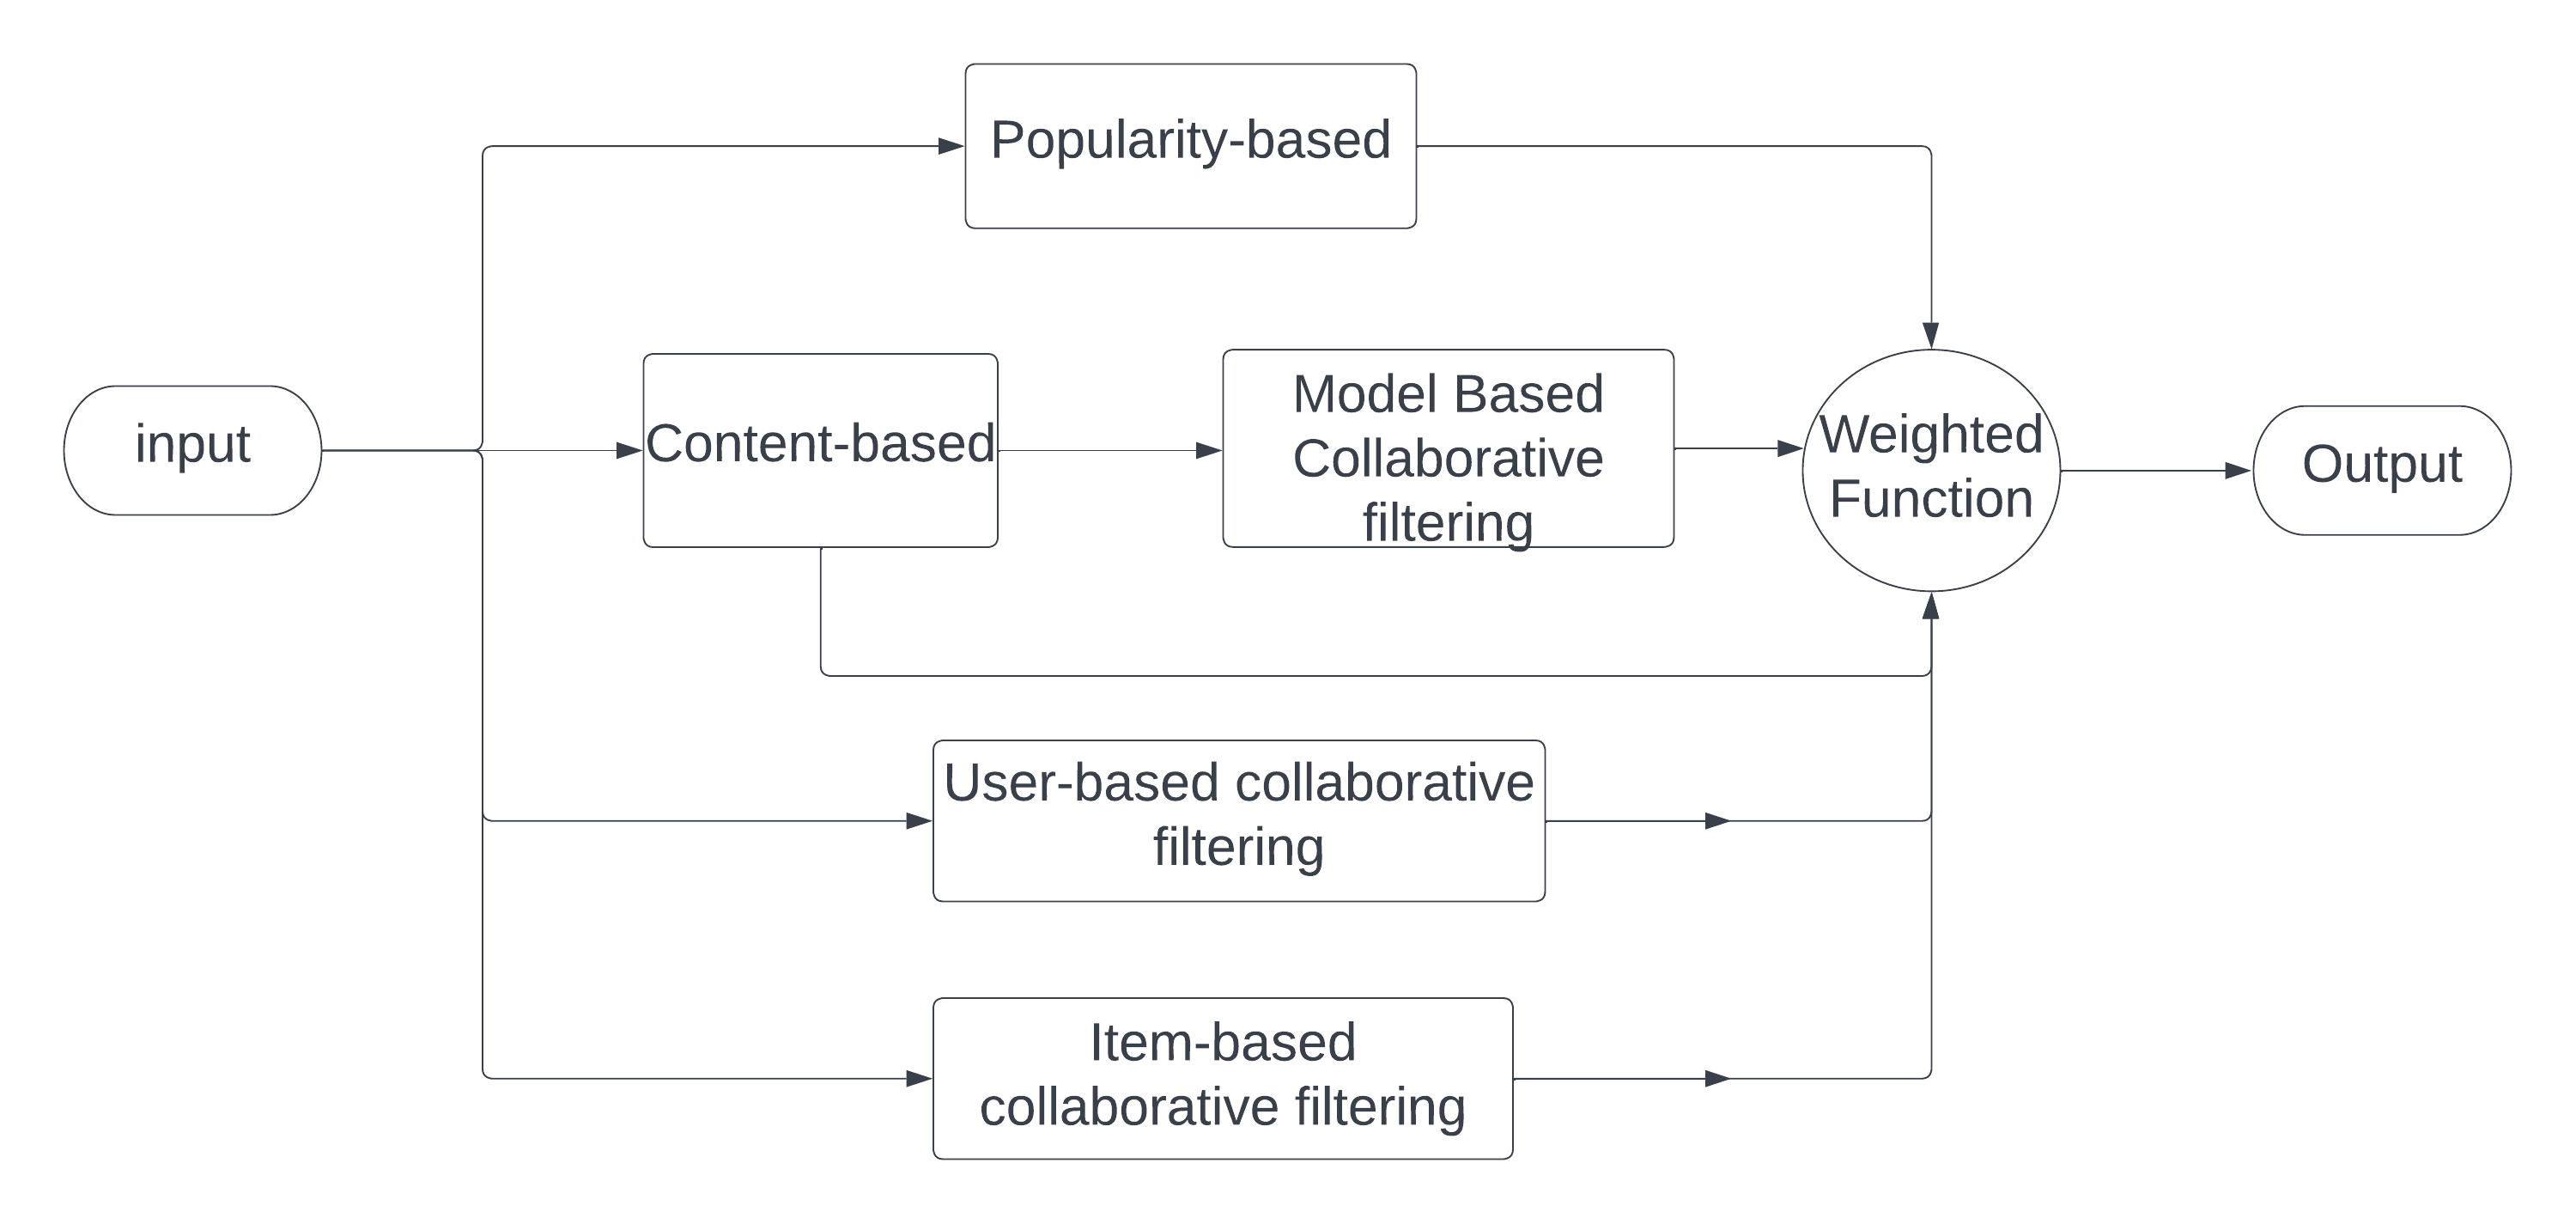
\includegraphics[scale = 0.15]{hybridd.png}
  \caption{Hybrid recommendation system design}
  \label{hybridd}
  \end{figure}
\\Firstly, the input, which is information gathered from our users, will be passed through the popularity-based system to get the ratings for their popularity.
\\In addition, the input will be fed into a content-based system to have ratings based on the similarity between users' preferences and posts' features. 
We also pass the output after the content-based system through model-based collaborative filtering (indicated by the red line) to improve performance. Notice we only allow the red path to go through when the content-based system finishes initialising the utility matrix for new users. It can be considered that we introduce a slight time delay at the beginning, and we do it because we need the content-based system to solve the cold-start problem in the model-based approach. The feedback (indicated by the green line) from the model-based sub-system is to solve the drawbacks in the content-based sub-system by providing a method to update the user parameter matrix.
\\Furthermore, the input will directly pass through an item-based collaborative filtering system in parallel with other sub-systems 
to have the ratings of posts based on the analysis of group behaviours. We can also introduce a user-based collaborative filtering system in parallel, but we abandoned it because of its poorer performance than the item-based filtering system.
\\Finally, after we have ratings after each design, we pass all the results into a weighting function, where we give weights to each sub-system output and then apply a linear combination.
The weight coefficients are calculated based on the performance and reliability of the sub-systems.
\\We only finished at the design stage, but in the future, we will use the RMSD metric to test our system performance because of its better penalty measures and low computational extensiveness. 

\section{Summary}
In this chapter, we discussed the different approaches to designing the recommendation system and analysed the applicability of every approach to our design. For each approach, we also identify some major challenges we may face and come up with some possible solutions we can apply to solve them. Finally, we created our own structure design of the recommendation engine, a hybrid system with different sub-systems connected in series and parallel. And the design is based on the principles of using different approaches to solve the drawbacks of each other. Currently, we have only finished the stage of designing the structure of the recommendation engine. However, in the future, we will perform tests of the performance of our design after we finish the programming and keep updating our design by trying new system approaches. Recommendation engine design is only one of the key elements in UX design during the whole project pipeline. In the next chapter, we will dive deeper into the back-end design of our primary app function which is chord generation, and it will discuss the first stage - Audio Pre-processing.

